\begin{figure}[t]
  \hspace{0.05\textwidth}%
  \begin{subfigure}[b]{\textwidth}
    \tikzstyle{legend-point}=[circle, inner sep=2pt]
    \definecolor{GraphBlue}{HTML}{6c8abd}
    \definecolor{GraphGreen}{HTML}{73b584}
    \definecolor{GraphRed}{HTML}{d07175}
    \definecolor{GraphPurple}{HTML}{8172b2}
    \definecolor{GraphYellow}{HTML}{ccb974}
    
    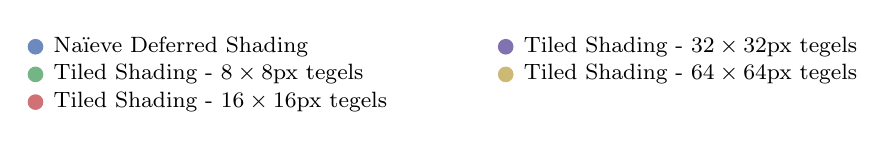
\begin{tikzpicture}
      \node (legend:1) at (0.1\textwidth,   0pt) [legend-point, fill={GraphBlue},  label=right:{\footnotesize Na\"ieve Deferred Shading}] {};
      \node (legend:2) at (0.1\textwidth, -10pt) [legend-point, fill={GraphGreen}, label=right:{\footnotesize Tiled Shading - $8 \times 8$px tegels}] {};
      \node (legend:3) at (0.1\textwidth, -20pt) [legend-point, fill={GraphRed},   label=right:{\footnotesize Tiled Shading - $16 \times 16$px tegels}] {};

      \node (legend:4) at (0.5925\textwidth,  -0pt) [legend-point, fill={GraphPurple}, label=right:{\footnotesize Tiled Shading - $32 \times 32$px tegels}] {};
      \node (legend:5) at (0.5925\textwidth, -10pt) [legend-point, fill={GraphYellow}, label=right:{\footnotesize Tiled Shading - $64 \times 64$px tegels}] {};
    \end{tikzpicture}
  \end{subfigure}\hfill\\
  \begin{adjustbox}{minipage=\textwidth, scale=0.55}
    \begin{subfigure}[b]{0.8\textwidth}
      \centering
      \def\svgwidth{\textwidth}
      \input{./img/raw/ts-lc-frames/deferred/frames_320_spaceship-indoor.pdf_tex}
      \caption{Spaceship Indoor: $70$ lichten, $320^2$ pixels.}
      \label{fig:ts-lc-frames-deferred:indoor-low}
    \end{subfigure}
  \end{adjustbox}\hspace{-0.075\textwidth}  %
  %
  \begin{adjustbox}{minipage=\textwidth, scale=0.55}
    \begin{subfigure}[b]{0.8\textwidth}
      \centering
      \def\svgwidth{\textwidth}
      \input{./img/raw/ts-lc-frames/deferred/frames_2560_spaceship-indoor.pdf_tex}
      \caption{Spaceship Indoor: $1260$ lichten, $2560^2$ pixels.}
      \label{fig:ts-lc-frames-deferred:indoor-high}
    \end{subfigure}
  \end{adjustbox} \\
  %
  \begin{adjustbox}{minipage=\textwidth, scale=0.55}
    \begin{subfigure}[b]{0.8\textwidth}
      \centering
      \def\svgwidth{\textwidth}
      \input{./img/raw/ts-lc-frames/deferred/frames_320_pipers-alley.pdf_tex}
      \caption{Piper's Alley: $58$ lichten, $320^2$ pixels.}
      \label{fig:ts-lc-frames-deferred:alley-low}
    \end{subfigure}
  \end{adjustbox}\hspace{-0.075\textwidth}  %
  %
  \begin{adjustbox}{minipage=\textwidth, scale=0.55}
    \begin{subfigure}[b]{0.8\textwidth}
      \centering
      \def\svgwidth{\textwidth}
      \input{./img/raw/ts-lc-frames/deferred/frames_2560_pipers-alley.pdf_tex}
      \caption{Piper's Alley: $1044$ lichten, $2560^2$ pixels.}
      \label{fig:ts-lc-frames-deferred:alley-high}
    \end{subfigure}
  \end{adjustbox} \\
  %
  \begin{adjustbox}{minipage=\textwidth, scale=0.55}
    \begin{subfigure}[b]{0.8\textwidth}
      \centering
      \def\svgwidth{\textwidth}
      \input{./img/raw/ts-lc-frames/deferred/frames_320_ziggurat-city.pdf_tex}
      \caption{Ziggurat City: $65$ lichten, $320^2$ pixels.}
      \label{fig:ts-lc-frames-deferred:city-low}
    \end{subfigure}
  \end{adjustbox}\hspace{-0.075\textwidth}  %
  %
  \begin{adjustbox}{minipage=\textwidth, scale=0.55}
    \begin{subfigure}[b]{0.8\textwidth}
      \centering
      \def\svgwidth{\textwidth}
      \input{./img/raw/ts-lc-frames/deferred/frames_2560_ziggurat-city.pdf_tex}
      \caption{Ziggurat City: $1170$ lichten, $2560^2$ pixels.}
      \label{fig:ts-lc-frames-deferred:city-high}
    \end{subfigure}
  \end{adjustbox}
  \caption{Overzicht van het aantal lichtberekeningen per frame voor Deferred Shading
           voor de drie testsc\'enes bij verschillende resoluties en aantallen
           lichten.}
  \label{fig:ts-lc-frames-deferred}
\end{figure}

